\documentclass[journal,a4paper]{IEEEtran}

\usepackage{algorithm}
\usepackage{algorithmic}

\usepackage{pgfplots}
\pgfplotsset{compat=1.9}

\usepackage[british]{babel}

\begin{document}

\title{An Adaptive Prefetcher Based on Delta-Correlating Prediction Tables and Reference Prediction Tables}
\author{Olav-Emil Eiksund, Christopher Lohne, Kristian Klomsten Skordal}
\maketitle

\begin{abstract}
This article describes an algorithm for L2 prefetching that combines the use of
delta-correlating prediction tables (DCPT) and reference prediction tables (RPT)
in order to get improved prefetcher accuracy, and thus better performance, under
varying conditions.

Under our simulated conditions, an average speedup of 7.6~\% was observed as
compared to using no prefetcher.
\end{abstract}

\section{Introduction}
\IEEEPARstart{A}{s} modern processors continue to get faster each year, memory speeds are not
increasing at the same rate, causing there to be a gap between memory and CPU speed.
When running applications, processors require data to be quickly
loaded from memory. When the required data is available in cache, the processor
has instant access to it, whereas a cache miss can cause delays as the neccessary
data is retrieved from random access memory.

By predicting what data the processor is going to need in the future, the
data can be transferred beforehand, reducing the risk of processor stalls and
unnecessary delays. There are many challenges connected to predicting what
data a processor is going to access, which has led to the development of a
multitude of algorithms, ranging from simple sequential prefetchers to more
complex pattern matching algorithms.

This paper describes the combination of two related pattern-matching approaches
to prefetching, reference prediction tables and delta-correlating prediction
tables, by using their accuracy to try to use the algorithm that gives the best
results in a given situation. The prefetcher implementation adheres to certain
limitations: it can only use 8~kB of memory and must be implemented in C or C++.

\section{Background}

\subsection{Reference Prediction Table}
Reference Prediction Tables, RPT, is an
efficient, yet lightweight, prefetcher heuristic. It requires little storage
and offers decent accuracy. The prefetcher consists of a table where each
entry contains the PC and last address of a miss instruction, a stride or
delta field, and a state field. The PC identifies the instruction causing
the miss, the last address is updated with the target address on every miss
and the delta is the difference between the previous and current last address.

On the first miss the entry is created and the state is set to initial. On
the second miss the delta is computed and the state is set to training. If
on any miss in the training state the new delta matches the old one, the
state is set to prefetching, and as long as the delta matches, it is used
to issue prefetches for $\textrm{last address} + \textrm{delta}$\cite{rpt}.

\subsection{Program Counter/Delta Correlation Prefetching}
Program Counter/Delta Correlation Prefetching, PC/DT, is an approach
proposed by K. J. Nesbit and J. E. Smith, in which all hits or misses
to a prefetched cache block are recorded in a global history buffer, GHB. It has
a PC indexed table of pointers into the GHB, that points to the last miss of an
instruction. The heuristic then calculates the deltas between miss addresses and
finds patterns in these to guess what will be accessed at the next memory access\cite{pcdc}.

\subsection{Delta-Correlating Prediction Tables}
An improvement over RPT, delta-correlating prediction tables, DCPT, uses the same principles.
It combines the tables of the RPT with delta correlation from the PC/DC heuristic.
The entry for the PC location is extended to include a circular buffer of $n$ deltas
with a delta pointer pointing to the head. The entry also includes a last prefetch field.
While it requires more space than the RPT, it is also more accurate. It manages to make
use of delta correlation without doing the expensive pointer chasing found in the PC/DC heuristic.

On each miss, instead of overwriting the delta as in RPT, the delta is added to
the circular buffer. The buffer is then traversed in reverse, searching for
matches for the last two deltas. The heuristic assumes that the same pattern is currently being
executed, and if matches are found, prefetch candidates are added to a Prefetch Candidate
Buffer for every delta from the match and up to the head of the circular buffer.

The prefetch candidates in the prefetch candidate buffer is then filtered, by checking
if any of the candidates match the last prefetch field, which causes all the candidates
up to that point to be cleared to avoid duplicate prefetches. Entries in the prefetch
candidate buffer are then checked to confirm that none of them are already in the cache
or already scheduled for prefetching. The last prefetch field is then updated with the
address issued for prefetch\cite{dcpt}.

\subsection{Delta-Correlating Prediction Tables with Partial Matching.}
A further improvement is described in \cite{dcptp}. The heuristic uses partial matching
when checking the address deltas, meaning that only the $n$ most significant bits are used.
While this is a small change from the regular DCPT, it allows for more complex patterns
to be captured while using the same amount of storage. Reducing spatial resolution this way
also increases the probability of cache pollution, and for this reason it is important that
a good value for n is found, that provides a balance between coverage and accuracy.

\section{Prefetcher Description}
The implemented prefetcher combines an RPT and a DCPT-P prefetcher and
switches between them in order to achieve the highest possible performance.
Both the DCPT and RPT implementation uses 22 bit deltas and partial matching
which masks the lower 8 bits of the deltas. For the prefetcher to use less
than 8~kB of memory, the DCPT-P table contains 42 entries, and the RPT
table contains 128 entries.

The algorithms are run alternatively and their accuracy is tracked.
At a predefined number of cache misses, an algorithm decides if the
currently running prefetcher algorithm should be switched. The switching
algorithm gives preference to the prefetcher algorithm having the highest
accuracy when deciding which algorithm to switch to, but is designed to allow
the other algorithm to run as well, to accomodate changes in the running
program environment.

The switching algorithm works by first using a random number generator to
choose a number between 0 and 100. Then, the accuracy of the algorithm with the
highest accuracy is multiplied by 100, giving the percentage accuracy of the
algorithm. This is then used to choose the algorithm to switch to; if the randomly
selected number is lower than or equal to the percentage accuracy of the highest
performing algorithm, that algorithm is selected, otherwise the other algorithm
is selected. The algorithm is illustrated in figure \ref{fig:switching}.

\begin{figure}[!h]
	\caption{Algorithm for switching between prefetchers}
	\label{fig:switching}
	\centering

	\begin{algorithmic}[1]
		\STATE $R \leftarrow \textrm{rand(0, 100)}$
		\IF{DCPT-P has higher accuracy}
			\IF{$\textrm{DCPT.accuracy} * 100 <= R$}
				\STATE $\textrm{Algorithm} \leftarrow \textrm{DCPT}$
			\ELSE
				\STATE $\textrm{Algorithm} \leftarrow \textrm{RPT}$
			\ENDIF
		\ELSIF{RPT has higher accuracy}
			\IF{$\textrm{RPT.accuracy} * 100 <= R$}
				\STATE $\textrm{Algorithm} \leftarrow \textrm{RPT}$
			\ELSE
				\STATE $\textrm{Algorithm} \leftarrow \textrm{DCPT}$
			\ENDIF
		\ENDIF
	\end{algorithmic}
\end{figure}

\section{Methodology}
In order to measure the performance of the prefetcher, the speedup compared to
using no prefetcher is measured. The speedup is then compared to the speedups
obtained by using only an RPT and only a DCPT-P prefetcher.

The prefetcher in this paper is tested on a M5 simulator system with a subset of
SPEC CPU2000 benchmark. The M5 simulator is a software platform that allows
simulating a complete hardware system. The simulated CPU is an Alpha 21264, which
is an out-of-order processor. The memory settings used for our simulations are shown
in table \ref{tab:simsetup}. There is no prefetching for the L1 cache. Statistics
were gathered after fast-forwarding $10^7$ instructions.

\begin{table}[h]
	\caption{Simulator setup\cite{userman}}
	\label{tab:simsetup}
	\centering

	\begin{tabular}{|l|l|}
		\hline
		L1 data cache & 64~kb \\
		L1 instruction cache & 32~kb \\
		L2 cache size & 1~Mb \\
		Memory bus width & 400~MHz \\
		Memory latency & 30~ns \\
		\hline
	\end{tabular}
\end{table}

The simulations were run on the Kongull computer cluster at the Norwegian University
of Science and Technology. The cluster consists of 107 nodes with two six core AMD
Opteron 2431 processors on each node\cite{kongull}. A script was used to run a subset
of the SPEC CPU2000 benchmark and obtain timing results and comparisons for the various
tests.

\section{Results}
The measured speedup compared to pure RPT and DCPT-P implementations are presented in
figure \ref{fig:results}. The best speedup can be observed in the ammp test, where
our speedup is almost 3 times the speedup of using a pure DCPT-P prefetcher. The
average speedup, using harmonic mean, was measured to be 7.6~\%.

\begin{figure}
	\caption{Comparison of RPT, DCPT-P and our prefetcher}
	\label{fig:results}
	\centering

	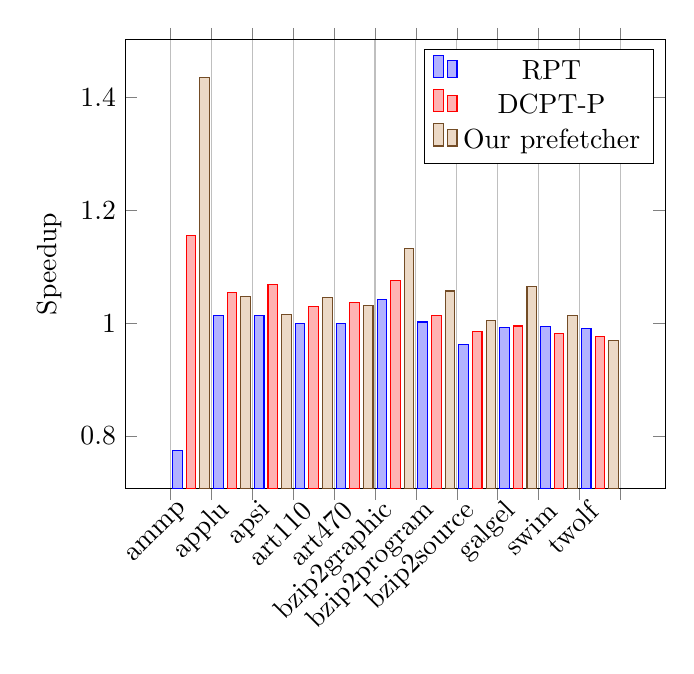
\begin{tikzpicture}
		\begin{axis}[
			ylabel=Speedup,
			ybar,
			symbolic x coords={ammp,applu,apsi,art110,art470,bzip2graphic,bzip2program,bzip2source,galgel,swim,twolf,wupwise},
			xtick=data,
			x tick label style={rotate=45,anchor=east},
			ybar interval=0.7
		]
			\addplot coordinates {(ammp,0.774) (applu,1.013) (apsi,1.014) (art110,0.999) (art470,0.999) (bzip2graphic,1.042) (bzip2program,1.002) (bzip2source,0.962) (galgel,0.993) (swim,0.994) (twolf,0.990) (wupwise,1.001)};
			\addplot coordinates {(ammp,1.155) (applu,1.054) (apsi,1.068) (art110,1.030) (art470,1.037) (bzip2graphic,1.075) (bzip2program,1.014) (bzip2source,0.986) (galgel,0.995) (swim,0.982) (twolf,0.976) (wupwise,1.142)};
			\addplot coordinates {(ammp,1.436) (applu,1.047) (apsi,1.016) (art110,1.046) (art470,1.032) (bzip2graphic,1.133) (bzip2program,1.057) (bzip2source,1.005) (galgel,1.065) (swim,1.014) (twolf,0.970) (wupwise,1.240)};
			\legend{RPT,DCPT-P,Our prefetcher}
		\end{axis}
	\end{tikzpicture}
\end{figure}

\section{Discussion}
The results show a small average improvement over the pure RPT and DCPT-P prefetchers
in all tests except the \emph{ammp} benchmark.

The reason for this relatively small improvement is probably that the RPT and DCPT-P
prefetchers does not produce very different results when run separately, which is not
surprising when considering that DCPT is basically RPT with more history.

\section{Future Work}
In order for the performance to increase further, it could be interesting to see the
results of combining other, more dissimilar algorithms, which may make the prefetcher
perform even better in varying conditions.

There are also many possibilities for tweaking the switching algorithm. One such
possibility is allowing the DCPT-P prefetcher to run in longer intervals than the
RPT prefetcher, since the DCPT-P prefetcher needs more historical data than the RPT.

The interval at which the switching is done also presents an opportunity for
experimentation. In this implementation, the interval that produced the best
performance was determined experimentally to be each 1~000~000 accesses.

The parameters for the individual prefetchers can also be tuned, such as the number
of deltas, number of bits in the deltas, the bitmasks used in the partial matching
and the number of entries in the lookup tables for each algorithm.

\section{Conclusion}
By combining an RPT prefetcher with a DCPT-P prefetcher and switching between them at
predefined intervals, an improved, adaptive prefetcher was created, with a small speedup
improvement over using a pure RPT or DCPT-P prefetcher separately.

\begin{thebibliography}{1}
	\bibitem{rpt} T. F. Chen and J. L. Baer, \emph{Effective Hardware-Based Data Prefetching for High-Performance Processors} in \emph{IEEE Transactions on Computers}, issue 44, pp. 609--623, May 1995.
	\bibitem{pcdc} K. J. Nesbit and J. E. Smith, \emph{Data Cache Prefetching using a Global History Buffer} from the \emph{International Symposium on High-Performance Computer Architecture}, ISSN 1530-0897, 2004.
	\bibitem{dcpt} Magnues Jahre and Lasse Natvig, \emph{Storafe Efficient Hardware Prefetching using Delta Correlating Prediction Tables} in \emph{Data Prefetching Championships}, 200.9
	\bibitem{dcptp} Marius Grannes, Magnus Jahre and Lasse Natvig, \emph{Multi-Level Hardware Prefetching Using Low Complexity Delta Correlating Prediction Tables with Partial Matching}, 2010.
	\bibitem{userman} NTNU Computer Architecture Group, \emph{M5 Simulator System}, NTNU, 2014.
	\bibitem{kongull} NTNU High Performance Computing Group, \emph{Kongull Hardware}, https://www.hpc.ntnu.no/display/hpc/Kongull+Hardware.
\end{thebibliography}

\end{document}

